% 2009-10-20
\nr
\section{Bindungskr\"afte}

\begin{enumerate}
\item Bindung in Festkörpern
\begin{enumerate}
	\item Bindungstypen
	\item Bindungsenergie
\end{enumerate}
\item Fluktuationsbindung
\begin{enumerate}
	\item Van-der-Waals-Kräfte
	\item Lennard-Jones-Potential
	\item Edelgaskristalle
\end{enumerate}
\item Ionenbindung
\begin{enumerate}
	\item Bindungsenergie
	\item Inonenkristalle
\end{enumerate}
\item Kovalente Bindungen
\item Metallische Bindungen
\item Wasserstoffbrückenbindung
\end{enumerate}

Festkörperphysik $\to$ Eigenschaften fester Materialien \\
$\underbrace{ \text{Atomkerne}+\text{Elektronen} }_{10^{23}}$

\subsection{Klassen von Festkörpern}
\begin{itemize}
\item Isolatoren
\item Halbleiter
\item Metalle
\item Supraleiter
\end{itemize}

\subsection{Fundamentale Konzepte}
\begin{itemize}
\item Schrödingergleichung
\item Pauli-Prinzip
\item Coulombsche-Wechselwirkung
\item Maxwellgleichungen
\item Statistische Mechanik
\end{itemize}


\begin{tabbing}
\qquad Unterschiedliche Atomare \=Ordnung \\ 
 \qquad $\swarrow$ \> $\searrow$\qquad \\ 
 idelale Kristalle\>ideale amorphe Festkörper 
\end{tabbing} 

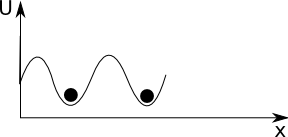
\includegraphics[scale=1]{images/2009-10-20-potentialberge.png}
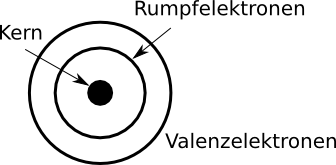
\includegraphics[scale=1]{images/2009-10-20-atomaufbau.png}

\subsection{5 Bindungstypen}
\begin{enumerate}
\item Fluaktions-Bindung
\item Ionenbindung
\item Kovalente-Bingungen
\item metallische Bindungen
\item Wasserstoffbrückenbindung
\end{enumerate}

\subsection{zweite Periode}
\begin{tabular}[b]{|c|c|c|c|c|c|c|c|c|}
\hline & Li & Be & B & C & $\text{N}_2$ & $\text{O}_2$ & $\text{F}_2$ & Ne \\ 
\hline Bindungsenergie $\nicefrac{\text{eV}}{\text{Atom}}$ & 1,6 & 3,3 & 5,8 & 7,4 & 4,9 & 2,6 & 0,8 & 0,02 \\ 
Schmelztemperatur K & 453 & 1560 & 2348 & 4765 & 62 & 54 & 53 & 24 \\ 
\hline\multicolumn{5}{c}{metall. charakter. Bindung$\searrow$ \quad $\nearrow$kovalente}  &\multicolumn{3}{c}{$\underbrace{\phantom{\qquad\qquad\qquad}}_{\text{Molekülkristalle}}$} \\ 
\end{tabular} 

Potential (Abstoßung) zwischen neutralen Atomen (Molekülen) mit abgeschlossener Elektronenschale

\includegraphics[scale=1]{images/2009-10-20-potential.png}
$E_1 \sim \dfrac{P_1}{P_2},\, P_2 \sim E_1$

$\phi (r)=\dfrac{A}{r^m},\, m=12$ oder $\phi(r)=A^\prime \text{e}^{\nicefrac{r}{\rho}}$

\subsection{Van-der-Waals-Bindung}

\includegraphics[scale=1]{images/2009-10-20-van_der_waals_bindung.png}


\begin{eqnarray}
\varphi(r) & \sim & \dfrac{\vec{P}_1\vec{P}_2}{r^3}-\dfrac{3(\vec{P}_1\vec{r})(\vec{P}_2\vec{r})}{r^5} \notag \\
\vec{P}_1 \parallel \vec{P}_2 \to \varphi(r) & = & -\dfrac{2P_1 P_2}{r^3} \notag \\
\varphi & \sim & -\dfrac{P_1 P_2}{r^3} \sim \dfrac{1}{r^6}\label{eq:van-der-waal-potential}
\end{eqnarray}
(\ref{eq:van-der-waal-potential}) heißt Van-der-Waal-Potential

$$\varphi(r)=\dfrac{A}{r^{12}}-\dfrac{B}{r^6}\equiv \underbrace{4\varepsilon\left[\left(\dfrac{\sigma}{r}\right)^{12}-\left(\dfrac{\sigma}{r}\right)^6\right]}_{\text{Lennard-Jones-Potential}} \qquad A=4\varepsilon \sigma^{12},\;B=4\varepsilon \sigma^6$$